
        \documentclass[addpoints,spanish, 12pt,a4paper]{exam}
        %\documentclass[answers, spanish, 12pt,a4paper]{exam}
        
        \pointpoints{punto}{puntos}
        \hpword{Puntos:}
        \vpword{Puntos:}
        \htword{Total}
        \vtword{Total}
        \hsword{Resultado:}
        \hqword{Ejercicio:}
        \vqword{Ejercicio:}

        \usepackage[utf8]{inputenc}
        \usepackage[spanish]{babel}
        \usepackage{eurosym}
        %\usepackage[spanish,es-lcroman, es-tabla, es-noshorthands]{babel}


        \usepackage[margin=1in]{geometry}
        \usepackage{amsmath,amssymb}
        \usepackage{multicol, xparse}

        \usepackage{yhmath}

        \usepackage{verbatim}
        %\usepackage{pstricks}


        \usepackage{graphicx}
        \graphicspath{{../img/}}




        \let\multicolmulticols\multicols
        \let\endmulticolmulticols\endmulticols
        \RenewDocumentEnvironment{multicols}{mO{}}
         {%
          \ifnum#1=1
            #2%
          \else % More than 1 column
            \multicolmulticols{#1}[#2]
          \fi
         }
         {%
          \ifnum#1=1
          \else % More than 1 column
            \endmulticolmulticols
          \fi
         }
        \renewcommand{\solutiontitle}{\noindent\textbf{Sol:}\enspace}

        \newcommand{\samedir}{\mathbin{\!/\mkern-5mu/\!}}

        \newcommand{\class}{1º Bachillerato}
        \newcommand{\examdate}{\today}

        %\newcommand{\tipo}{A}


        \newcommand{\timelimit}{50 minutos}

        \renewcommand{\solutiontitle}{\noindent\textbf{Solución:}\enspace}


        \pagestyle{head}
        \firstpageheader{
\includegraphics[width=0.2\columnwidth]{header_left}}{\textbf{Departamento de Matemáticas\linebreak \class}\linebreak \examnum}{
\includegraphics[width=0.1\columnwidth]{header_right}}
        \runningheader{\class}{\examnum}{Página \thepage\ of \numpages}
        \runningheadrule
        
        \pointsinrightmargin % Para poner las puntuaciones a la derecha. Se puede cambiar. Si se comenta, sale a la izquierda.
        \extrawidth{-2.4cm} %Un poquito más de margen por si ponemos textos largos.
        \marginpointname{ \emph{\points}}

        \printanswers
            \newcommand{\tipo}{l}\newcommand{\examnum}{Auto evaluación 2 - 1ª evaluación}
        \begin{document}
        \noindent
        \begin{tabular*}{\textwidth}{l @{\extracolsep{\fill}} r @{\extracolsep{6pt}} }
        \textbf{Nombre:} \makebox[3.5in]{\hrulefill} & \textbf{Fecha:}\makebox[1in]{\hrulefill} \\
         & \\
        \textbf{Tiempo: \timelimit} & Tipo: \tipo 
        \end{tabular*}
        \rule[2ex]{\textwidth}{2pt}
        Esta prueba tiene \numquestions\ ejercicios. La puntuación máxima es de \numpoints. 
        La nota final de la prueba será la parte proporcional de la puntuación obtenida sobre la puntuación máxima. 

        \begin{center}


        \addpoints
             %\gradetable[h][questions]
            \pointtable[h][questions]
        \end{center}

        \noindent
        \rule[2ex]{\textwidth}{2pt}

        \begin{questions}
        \question Efectúa simplificando el resultado si es posible:
        \begin{multicols}{1} 
        \begin{parts} \part[1]  $ \frac{\frac{x^2+2x+1}{x - 3}}{\frac{x+1}{x^2 -9 }} $  \begin{solution}  $ x^{2} + 4 x + 3 $  \end{solution} \part[1]  $ \frac{3x^2+1}{x^2+x}  - \frac{2x}{x+1} $  \begin{solution}  $ \frac{x^{2} + 1}{x^{2} + x} $  \end{solution}
        \end{parts}
        \end{multicols}
        \question Resuelve mediante expresiones algebraicas y Gauss:
        \begin{multicols}{1} 
        \begin{parts} \part[1] Se tienen 140 euros, en 20 billetes, unos de 5 euros y de 10 los restantes. 
    ¿Cuántos billetes hay de cada clase?  \begin{solution}  $ \left\{\begin{matrix}140=5x+10y\\ 20=x+y\\ \end{matrix}\right.  \rightarrow  \\\left[\begin{matrix}10 & 5 & 140\\0 & \frac{1}{2} & 6\end{matrix}\right] \rightarrow  \left \{ x : 12, \quad y : 8\right \} $  \end{solution} \part[1] En una clase los 2/3 del número de alumnas es igual a los 5/7 del número de alumnos. Si el número de
alumnas aumenta en 26, entonces es igual al doble del número de alumnos. ¿Cuántos alumnos y alumnas
tiene la clase?  \begin{solution}  $ \left\{\begin{matrix}\frac{2x}{3}=\frac{5y}{7}\\ x+26=2y\\ \end{matrix}\right.  \rightarrow  \\\left[\begin{matrix}- \frac{5}{7} & \frac{2}{3} & 0\\0 & \frac{13}{15} & 26\end{matrix}\right] \rightarrow  \left \{ x : 30, \quad y : 28\right \} $  \end{solution}
        \end{parts}
        \end{multicols}
        \question Discute y resuelve los sistemas:
        \begin{multicols}{1} 
        \begin{parts} \part[1]  $ \left\{\begin{matrix}x+y+z=1\\ x + 2y - z = 2\\ 2x +3y = 3\\ \end{matrix}\right. $  \begin{solution}  $ \left[\begin{matrix}1 & 1 & 1 & 1\\0 & -1 & -3 & 0\\0 & 0 & 0 & 0\end{matrix}\right] \rightarrow  \\ \left \{ x : - 3 z, \quad y : 2 z + 1\right \} $  \end{solution} \part[1]  $ \left\{\begin{matrix}\frac{x}{2} + \frac{y}{3} + \frac{z}{3} = -2\\ \frac{x}{3} - \frac{y}{2} + \frac{z}{3} = 2\\ \frac{x}{6} + \frac{y}{2} + \frac{z}{2} = 1\\ \end{matrix}\right. $  \begin{solution}  $ \left[\begin{matrix}\frac{1}{3} & \frac{1}{2} & \frac{1}{3} & -2\\0 & \frac{13}{12} & \frac{5}{6} & -1\\0 & 0 & \frac{35}{78} & \frac{45}{13}\end{matrix}\right] \rightarrow  \\ \left \{ x : - \frac{48}{7}, \quad y : - \frac{24}{7}, \quad z : \frac{54}{7}\right \} $  \end{solution}
        \end{parts}
        \end{multicols}
        \question Resuelve los siguientes sistemas de inecuaciones:
        \begin{multicols}{1} 
        \begin{parts} \part[1]  $ \left\{\begin{matrix}\frac{{x - 1}}{2} - \frac{{x + 3}}{3} \leq x\\ \frac{{4x - 2}}{4} - \frac{{x - 1}}{3} \geq x\end{matrix}\right. $  \begin{solution}  $ \left[- \frac{9}{5}, - \frac{1}{2}\right] $  \end{solution} \part[1]  $ \left\{\begin{matrix}{( {x - 1} )^2} - {( {x - 3} )^2} \leq 0\\x - 3( {x + 1}^2 ) \leq 3 \end{matrix}\right. $  \begin{solution}  $ \left(-\infty, 2\right] $  \end{solution}
        \end{parts}
        \end{multicols}
        \question Resuelve los siguientes sistemas de inecuaciones:
        \begin{multicols}{1} 
        \begin{parts} \part[1]  $ \left\{\begin{matrix}- 2 \leq x\\x \leq 2\\y \geq 4\\x + y - 1 \leq 0\\\end{matrix}\right. $  \begin{solution}    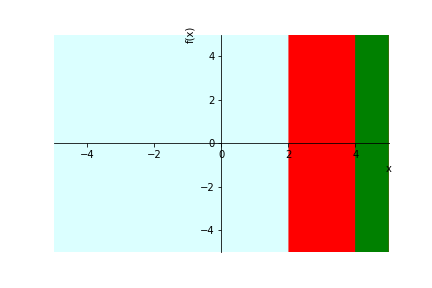
\includegraphics[width=1\columnwidth]{si4}   \end{solution} \part[1]  $ \left\{\begin{matrix}x \geq 0 \\0 \leq y\\y \leq 3\\x - 2y \leq 10\\x + y \geq 10\\\end{matrix}\right. $  \begin{solution}    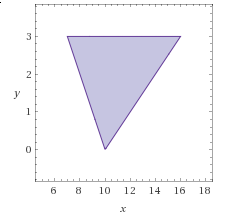
\includegraphics[width=1\columnwidth]{si5}   \end{solution}
        \end{parts}
        \end{multicols}
        \question Averigua el valor de x en los siguientes casos:
        \begin{multicols}{1} 
        \begin{parts} \part[1]  $ 2\log x - \log (x - 16) = 2 $  \begin{solution}  $ \left [ \right ] $  \end{solution} \part[1]  $ \log x + \log (50) = \log (1000) $  \begin{solution}  $ \left [ 20\right ] $  \end{solution}
        \end{parts}
        \end{multicols}
        \question Resuelve los siguientes sistemas:
        \begin{multicols}{1} 
        \begin{parts} \part[1]  $ \left\{\begin{matrix}\log x + \log y = 8 \\\log x - \log y = 2\end{matrix}\right. $  \begin{solution}  $ \left [ \left \{ x : 100000, \quad y : 1000\right \}\right ] $  \end{solution} \part[1]  $ \left\{\begin{matrix}3\log x - 2\log y = 10\\\log x + 3\log y = 7\end{matrix}\right. $  \begin{solution}  $ \left [ \left \{ x : 10000, \quad y : 10\right \}\right ] $  \end{solution}
        \end{parts}
        \end{multicols}
        
    \end{questions}
    \end{document}
    